\documentclass{article}
%\documentclass[aos,preprint]{imsart}
\usepackage{amsmath,amsfonts,amssymb,graphics,amscd}
\usepackage[square]{natbib}
\usepackage{hyperref}
\usepackage[normalem]{ulem}
\usepackage[parfill]{parskip}
\usepackage{graphicx}
\usepackage{inconsolata}
\usepackage{caption}
\usepackage{subcaption}
\usepackage{framed}
\usepackage{float}

\newcommand{\Prob}[1]{\ensuremath{\mathrm{Pr}\left( #1 \right) }}
\newcommand{\Expect}[1]{\ensuremath{\mathbb{E}\left[ #1 \right]}}
\newcommand{\ProcAlphabet}{\ensuremath{\mathcal{A}}}
\newcommand{\StateSet}{\ensuremath{\mathcal{S}}}
\newcommand{\indep}{\ensuremath{\rotatebox{90}{$\models$}}}
\newcommand{\synctime}{\ensuremath{\tau_{\mathrm{synch}}}}
\newcommand{\match}{\ensuremath{\mathrm{match}}}
\newcommand{\homog}{\ensuremath{\mathrm{homog}}}
\newcommand{\excisable}{\ensuremath{\mathrm{excisable}}}
\newtheorem{proposition}{Proposition}
\newtheorem{definition}{Definition}
\newtheorem{lemma}{Lemma}
\begin{document}

\title{ROCS Algorithm}
\author{Redrafted by Sam Stites}
\date{\LaTeX 'd \today}
\maketitle

\section{Phase I: Build the Parse Tree}

Notes:

\begin{itemize}

\item Building up a Parse tree is constrained by a max-length. Is there a way to
build up some of the parse tree, get information about the looping tree, then
continue building up the parse tree?
  \begin{itemize}
    \item This can probably be done by including \textit{non-terminal},
      \textit{non-looping} nodes. If they exist in the looping tree, more
      information is needed.
  \end{itemize}

\item instead of being \textit{given} an alphabet, we can build one as we
  iterate through the data.

\end{itemize}

\section{Phase II: Grow the Looping Tree}

See Appendix for definitions of {\bf match}, {\bf homogeneous}, and {\bf
excisable}.

\begin{leftbar}
\begin{enumerate}
\item Begin with a single node which matches the null prefix, i.e., everything.
  Set this to be a terminal node.
\item For each terminal node, check whether $w$ is homogeneous
  \begin{enumerate}
  \item If $\homog(w)$, leave $w$ alone.
  \item If $\neg\homog(w)$, delete $w$ from the set of terminal nodes (but
    leave its node in the tree).  For each symbol $a$ from the alphabet, add
    child nodes for each $aw$, unless that string does not occur in the input
    data.  For each created child node $aw$, check whether $aw=eq$ for some
    excisable prefix $e$ and suffix $q$.
    \begin{enumerate}
    \item If so, delete the node $aw$, and create a loop from $w$ to $q$ with
      the label $a$.
    \item If not \sout{(i.e., if $aw$ has no excisable prefix), check whether
      $\match(aw,r)$ for some existing terminal node $r$.} add $aw$ to the set
      of terminal nodes (edge set checks will happen during refinement).
      \begin{enumerate}
      \item \sout{If so, delete the node $aw$ and create an edge labeled $a$ from $w$
        to $r$.}
      \item \sout{If not, add $aw$ to the set of terminal nodes.}
      \end{enumerate}
    \end{enumerate}
  \end{enumerate}
\item Continue until all terminal nodes are homogeneous.
\end{enumerate}
\end{leftbar}


\section{Phase III: Refine the Looping Tree}

I propose that refinement be broken into two sub-phases: refinement of
loops and transistions and merging of edgesets.

\begin{leftbar}
\begin{tabbing}
  First, initialize a transition map from terminals to looping nodes.\\
  Next, refinement (same as before):\\
  Until \= (no change)\\
  \> for \= each terminal node $t$\\
  \> \> for \= each non-looping path $w$ to $t$\\
  \> \> \> for \= each symbol $a$ in the alphabet\\
  \> \> \> \> follow the path $wa$ in the tree\\
  \> \> \> \> if $wa$ \= leads to a terminal node, continue\\
  \> \> \> \> \>         {\bf and record in transition map}\\
  \> \> \> \> {\bf else if} \= ($==$ $wa$ does not lead to a terminal node)\\
  \> \> \> \> \> copy the sub-looping-tree rooted at (the node\\
  \> \> \> \> \> reached by) $wa$ to $t$, giving all terminal\\
  \> \> \> \> \> nodes the predictive distribution of $t$\\
  \> \> \> \> {\bf else break inner-most loop}
\end{tabbing}
\end{leftbar}

Now, merge edgesets:

\begin{leftbar}
\begin{tabbing}
  - Given \= a map of collected transitions \texttt{Map Terminal -> Node}\\
  \> - group collected transitions \textit{by the exact set of nodes transitioned to}\\
  \> \textit{\textbf{or by any transition subset found}}.\\
  - throw away the transitions and look only at the grouped terminals.\\
  - item iterate through each group\\
  \> - partition groups by checking for \textbf{matching} distributions\\
  - ignoring singleton groups, merge terminals into "edgesets"\\
  - if any merging occurred, restart refinement.\\
\end{tabbing}
\end{leftbar}

Merging terminals into edgesets by matching transitions and distributions gets
us out of the Tricky Hidden Markov Model situation, see edgecase from earlier
email. However, this causes us to break our logic in handling Holmes' and
Isabelle's flip machine (the original motivation for using looping trees). It
breaks down in the following manner.

\subsection{Fixing an Holmes-Isabelle issue}

Here is Holmes-Isabelle, a screenshot from the paper:

\begin{figure}[h!]
\centering
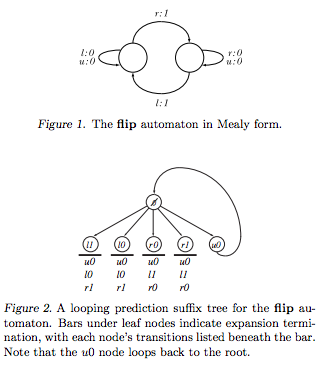
\includegraphics[width=50mm,scale=0.5]{imgs/flip-mealy.png}
\label{fig:method}
\end{figure}

And as constructed prior to the introduction of merging edgesets:

\begin{figure}[h!]
\centering
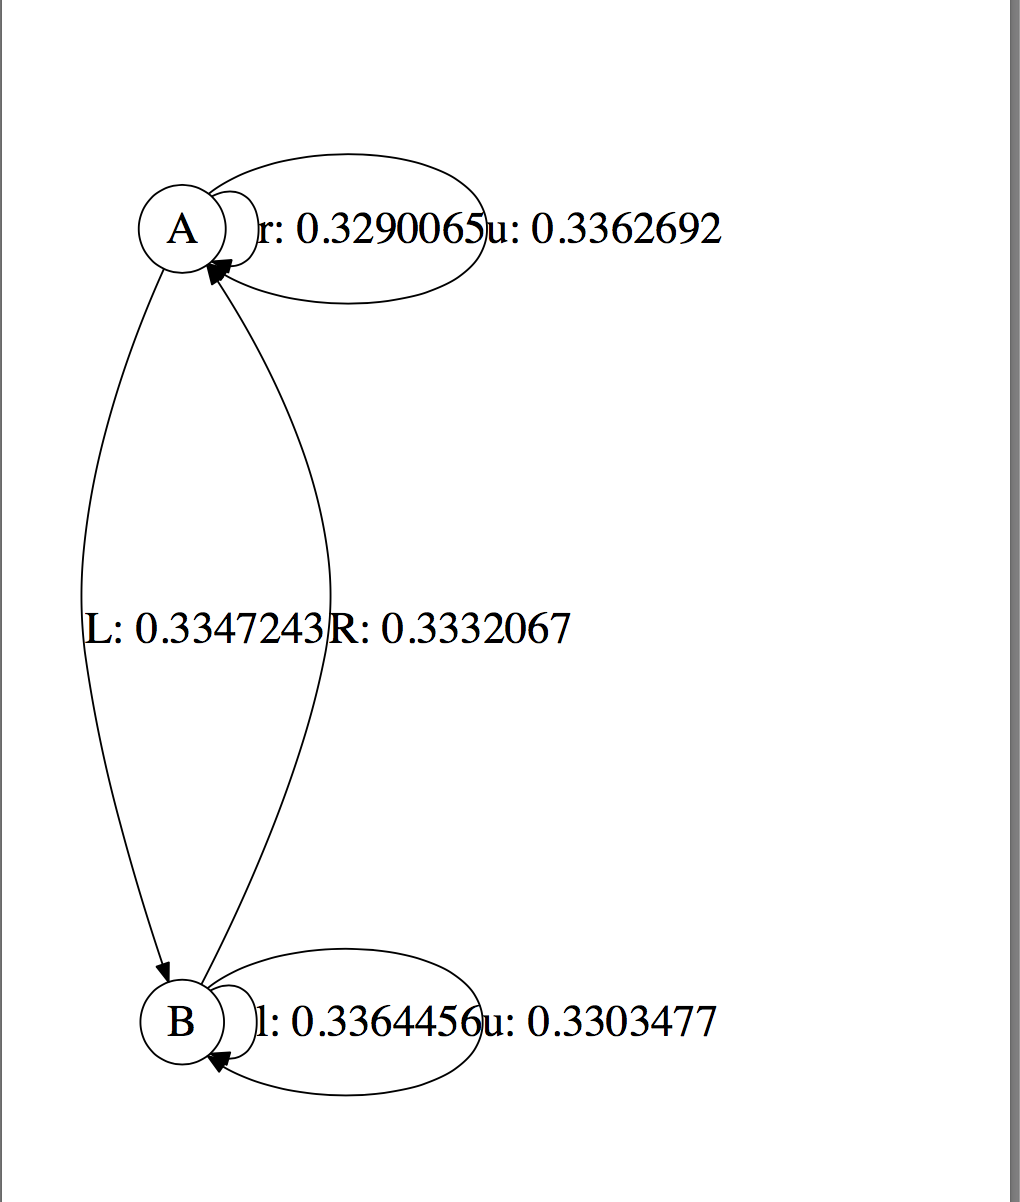
\includegraphics[width=50mm,scale=0.5]{imgs/flip-no-merge.png}
\label{fig:method}
\end{figure}


\newpage


In our algorithm, we build a looping tree with the following terminal nodes.
Note that the next-step distributions for an alphabet of {\tt [l, L, r, R, u]}

{\tt l: distribution of [0.33,0.0,0.0,0.33,0.34]}\\
\\
{\tt r: distribution of [0.0,0.34,0.33,0.0,0.33]}\\
\\
{\tt R: distribution of [0.0,0.33,0.33,0.0,0.34]}\\
\\
{\tt L: distribution of [0.34,0.0,0.0,0.34,0.32]}\\

Performing refinement, we get the following paths in our looping tree:

{\tt l + l -> l}\\
{\tt l + R -> R}\\
{\tt l + u -> l}\\
\\
{\tt r + L -> L}\\
{\tt r + r -> r}\\
{\tt r + u -> r}\\
\\
{\tt R + L -> L}\\
{\tt R + r -> r}\\
{\tt R + u -> R}\\
\\
{\tt L + l -> l}\\
{\tt L + R -> R}\\
{\tt L + u -> L}\\


which forms the following transition map:

{\tt l -> l}\\
{\tt l -> R}\\
\\
{\tt r -> L}\\
{\tt r -> r}\\
\\
{\tt R -> L}\\
{\tt R -> r}\\
{\tt R -> R}\\
\\
{\tt L -> l}\\
{\tt L -> R}\\
{\tt L -> L}\\

\newpage

Note that if we are to merge edgesets, we would find two groupings of
transitions: groups with distribution {\tt [0.33,0.0,0.0,0.33,0.34]} from {\tt l}
and {\tt L}, and groups with distribution {\tt [0.0,0.34,0.33,0.0,0.33]} from
{\tt r} and {\tt R}. However grouping by transitions, will result in each terminal
node having a unique transition map.

\begin{figure}[h!]
\centering
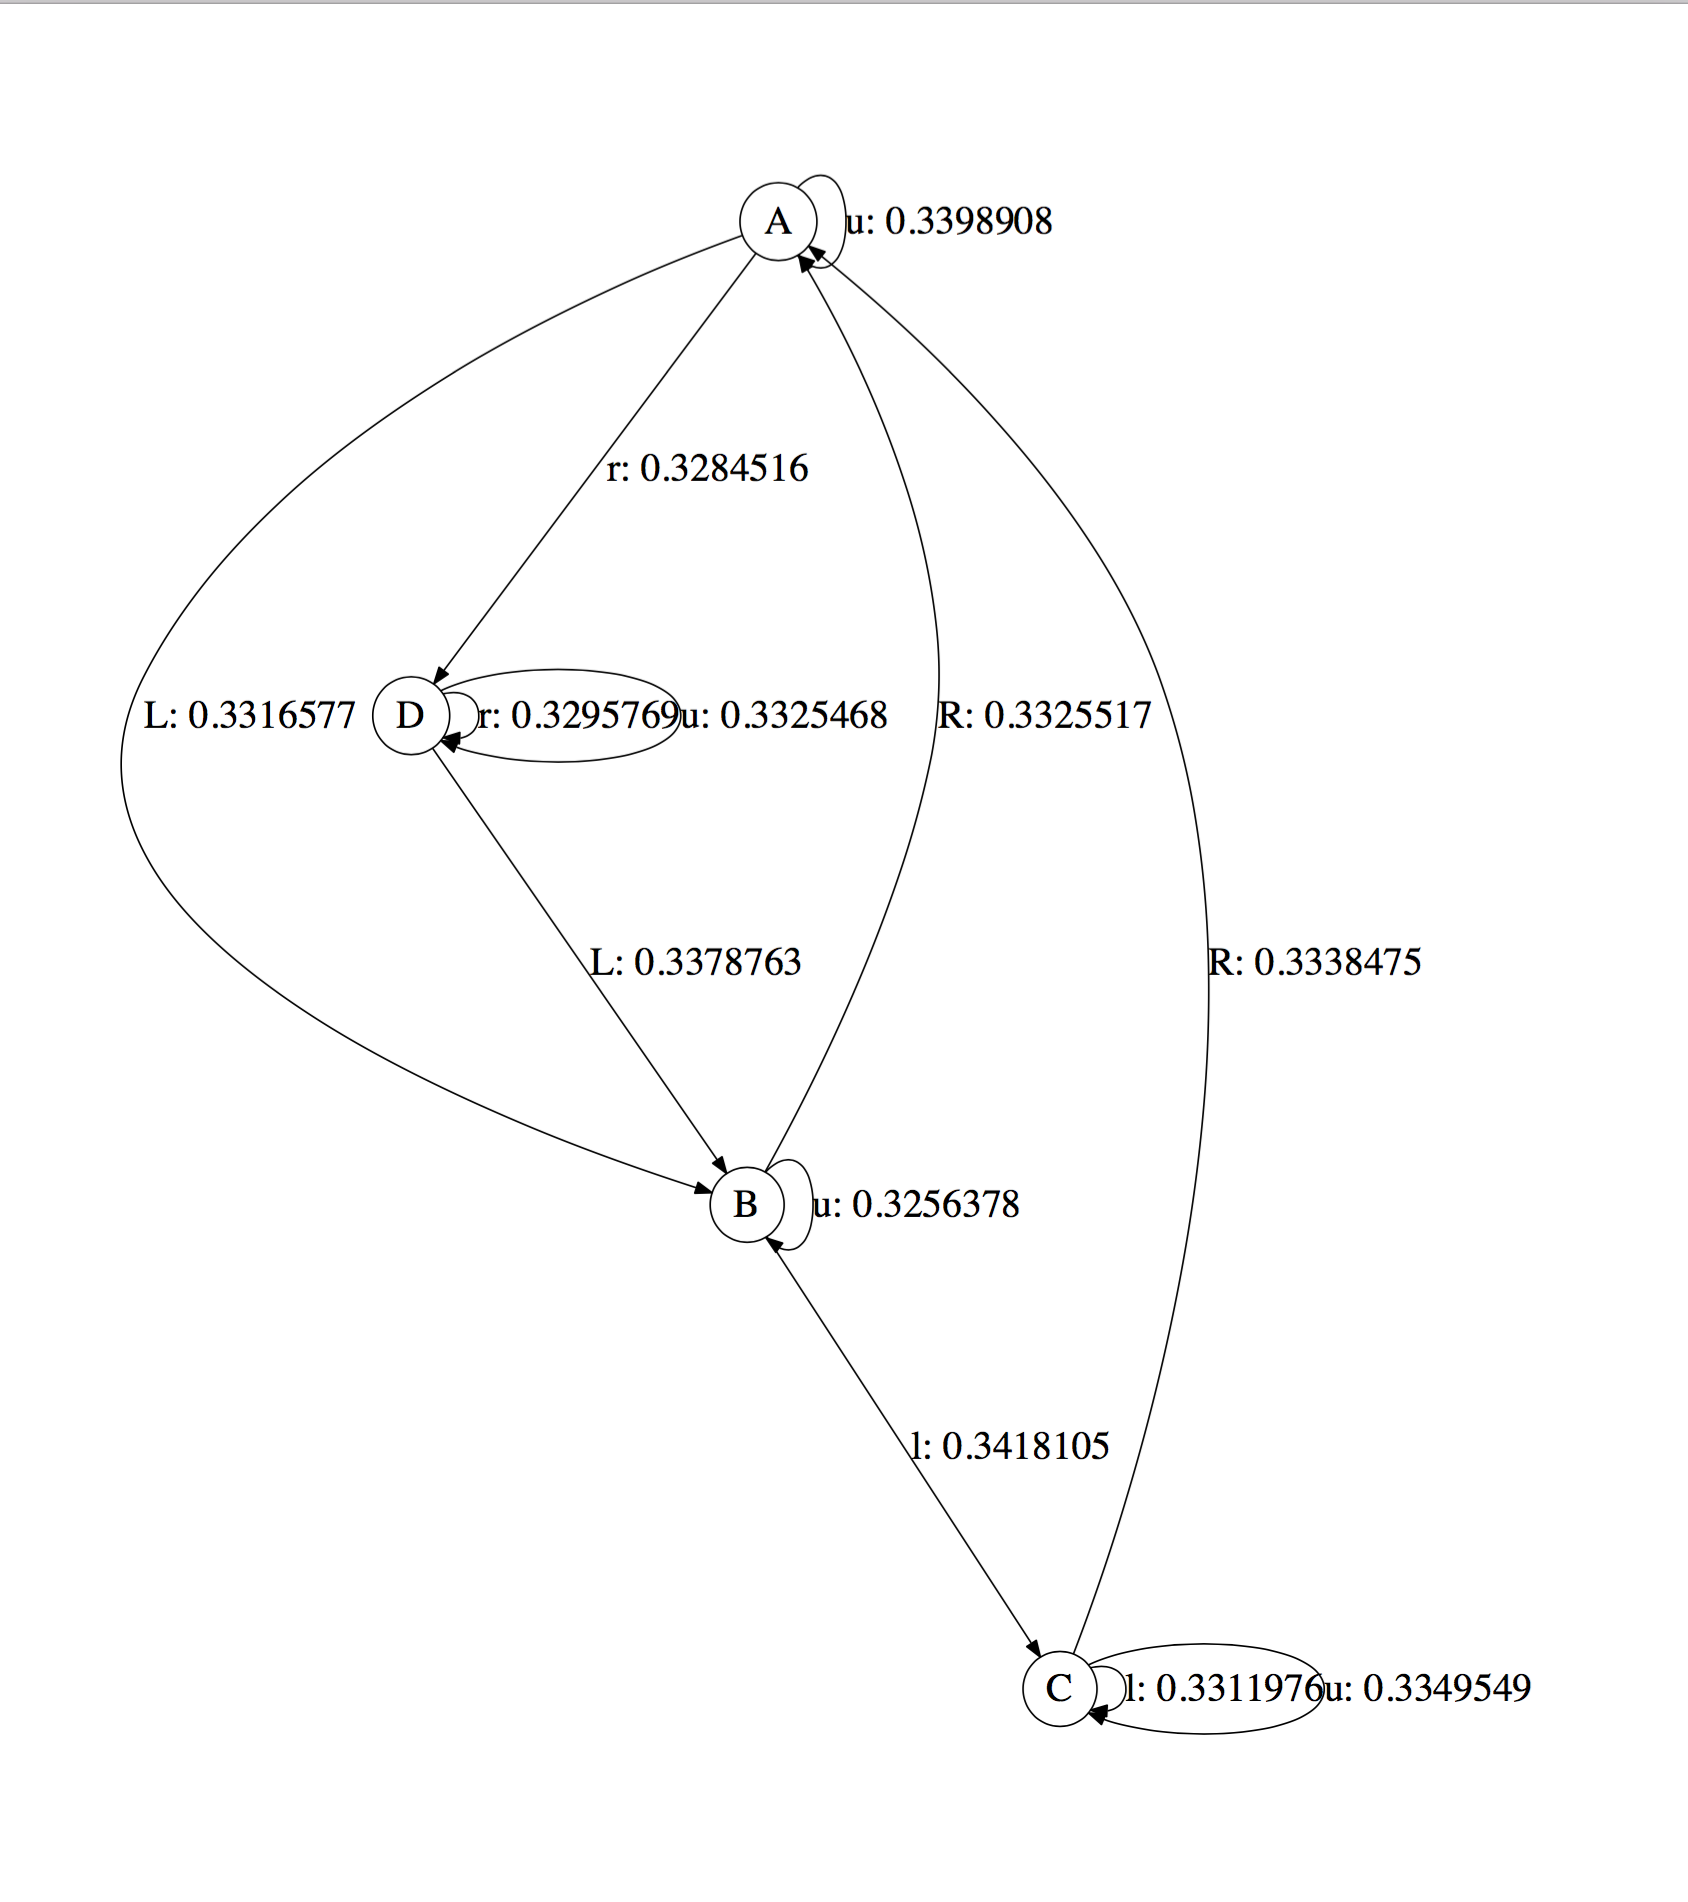
\includegraphics[width=75mm]{imgs/flip-merge.png}
\caption{post-refinement looping tree for flip machine with merging}
\label{fig:method}
\end{figure}

\newpage

This can be side-stepped by noticing how some terminals' (ie: {\tt l} and {\tt r})
transitions subset other terminals' transitions ({\tt L} and {\tt R},
respectively) and also have idential next-step distributions.

Using this new ruleset, we amend the first step of edgeset merging to group
transitions by the exact set of nodes transitioned to \textit{\textbf{or by any
transition subset found}}.

Doing so allows us to recover the discovery of a correct Isabelle-Holmes'
Flip machine, while also accounting for the Tricky Hidden Markov Model.


\begin{figure}[H]
\centering
\begin{subfigure}{.5\textwidth}
  \centering
  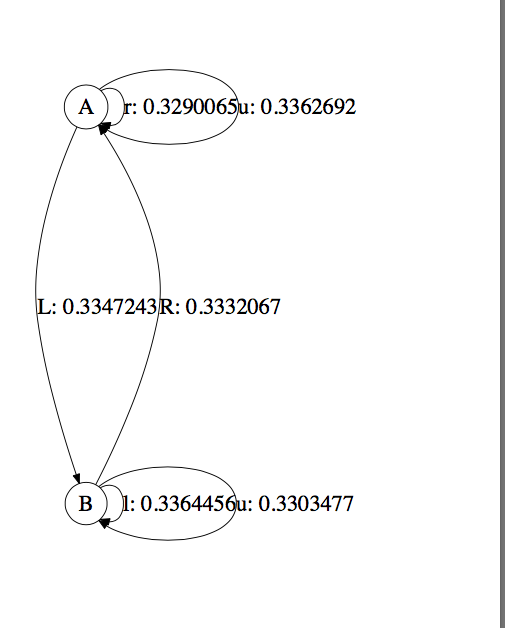
\includegraphics[width=50mm,scale=0.5]{imgs/flip-merge-subset.png}
  \caption{Flip Machine}
  \label{fig:sub1}
\end{subfigure}%
\begin{subfigure}{.5\textwidth}
  \centering
  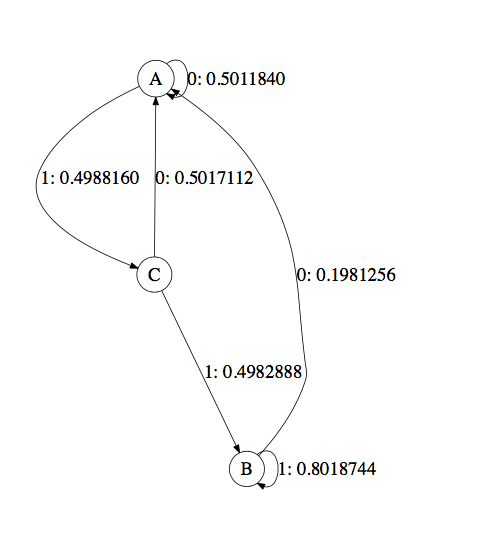
\includegraphics[width=50mm,scale=0.5]{imgs/TMD-subsetting.png}
  \caption{Tricky Hidden Markov Model}
  \label{fig:sub2}
\end{subfigure}
\caption{post-refinement looping tree for HMMs with merging of sets and subsets
of transitions}
\label{fig:test}
\end{figure}


\appendix

\section{Definitions}

\begin{itemize}
\item Two words $u$, $v$ {\bf match} iff they lead to the same prediction for
  the next step.  Write this $\match(u,v)$.
\item A word $w$ is {\bf homogeneous} iff, for any prefix $u$, $\match(w,uw)$.
  Write this $\homog(w)$.  This means earlier history is irrelevant,
  conditional on $w$.
\item If $w=eq$, then the prefix $e$ is {\bf excisable} from $w$ iff, for all
  prefixes $p$, $\match(peq, pq)$.  That is, inserting the extra history $e$
  before $q$ makes no difference to predictions.
\end{itemize}



\end{document}
